\section{Q1. How a transition system is built}
\label{sec:Q1}
%Does the report clearly describe how a transition system is being built? Which parts of the explanation are good? Which parts could be improved and how?

In order to build a transition system, one must specify which states are in the system. To explain the procedure properly, the section is divided into what the user does, and correspondingly what the program performs.

\subsection{Building the transition system: User}

When the user defines the transition system, each state must be specified. In particular; the new states number/id, if the new given state is an initial state, what the state's atomic propositions are, and which states it is connected to (the targets for the states edges). This is implemented with the given code fragment:

\begin{lstlisting}
ts.add(1, true, new String[] {"v"}, new int[] { 2 });
\end{lstlisting}

This arguments in the code is understood as:
\begin{enumerate}
\item Add the new state with state number (id) 1. 
\item The new state is set as initial state with the argument \textcolor{blue}{true}
\item The state has the atomic proposition \textsf{v}.
\item There is only one edge from this state. The target of the edge is state 2.
\end{enumerate}

An important thing to note, is that it is possible to create an edge to a state which is not yet implemented. \\

Once the transition system is built, it is possible to inspect the complete transition system by using
\begin{lstlisting}
ts.printStates(ctlTT());
\end{lstlisting}

which outputs all states in detail as seen in figure \ref{fig:stateprint}

\begin{figure}[H]
    \centering
    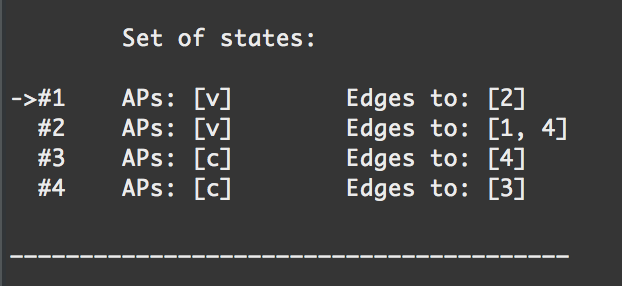
\includegraphics[width=0.4\textwidth]{fig/stateprinter.png}
    \caption{Output of implemented state printer. Shows initial state ($\rightarrow$), state id (\#), atomic propositions (APs) and targets of edges (Edges to). This example uses the transition system from the assignment description. This example will be used in later sections.}
    \label{fig:stateprint}
\end{figure}

This way the user can specify all details of the transition system and get confirmed that the system is correct.

\subsection{Building the transition system: Program}

An overview of the program itself is shown in the class diagram in figure \ref{fig:classdiagram}. \\


The class diagram shows, that when the user specifies the states in the system, they are called through methods in the initialized \texttt{TransitionSystem} object \texttt{ts}. Each time the user calls the \texttt{add($\hdots$)} method, the transition system instantiates a \texttt{State} object which is stored in the list \texttt{states} in the transition system. Each of the given arguments for the \texttt{add($\hdots$)} method are passed to the \texttt{State} constructor,\footnote{The arrays are made into lists for easy access to elements.} setting the corresponding parameters. \\ 

In order to display the specified transition system, the important details of each \texttt{State} in \texttt{states} are displayed in the console, making it possible to check if an error has occurred. \\

*Note: The program does not check whether the specified state number already exists for one of the states in the system. The consequence is, that if one deliberately creates non-unique states, the program may not act as expected. This aspect was not mentioned in the assignment and therefore not implemented in the program.

\begin{figure}[H]
    \centering
    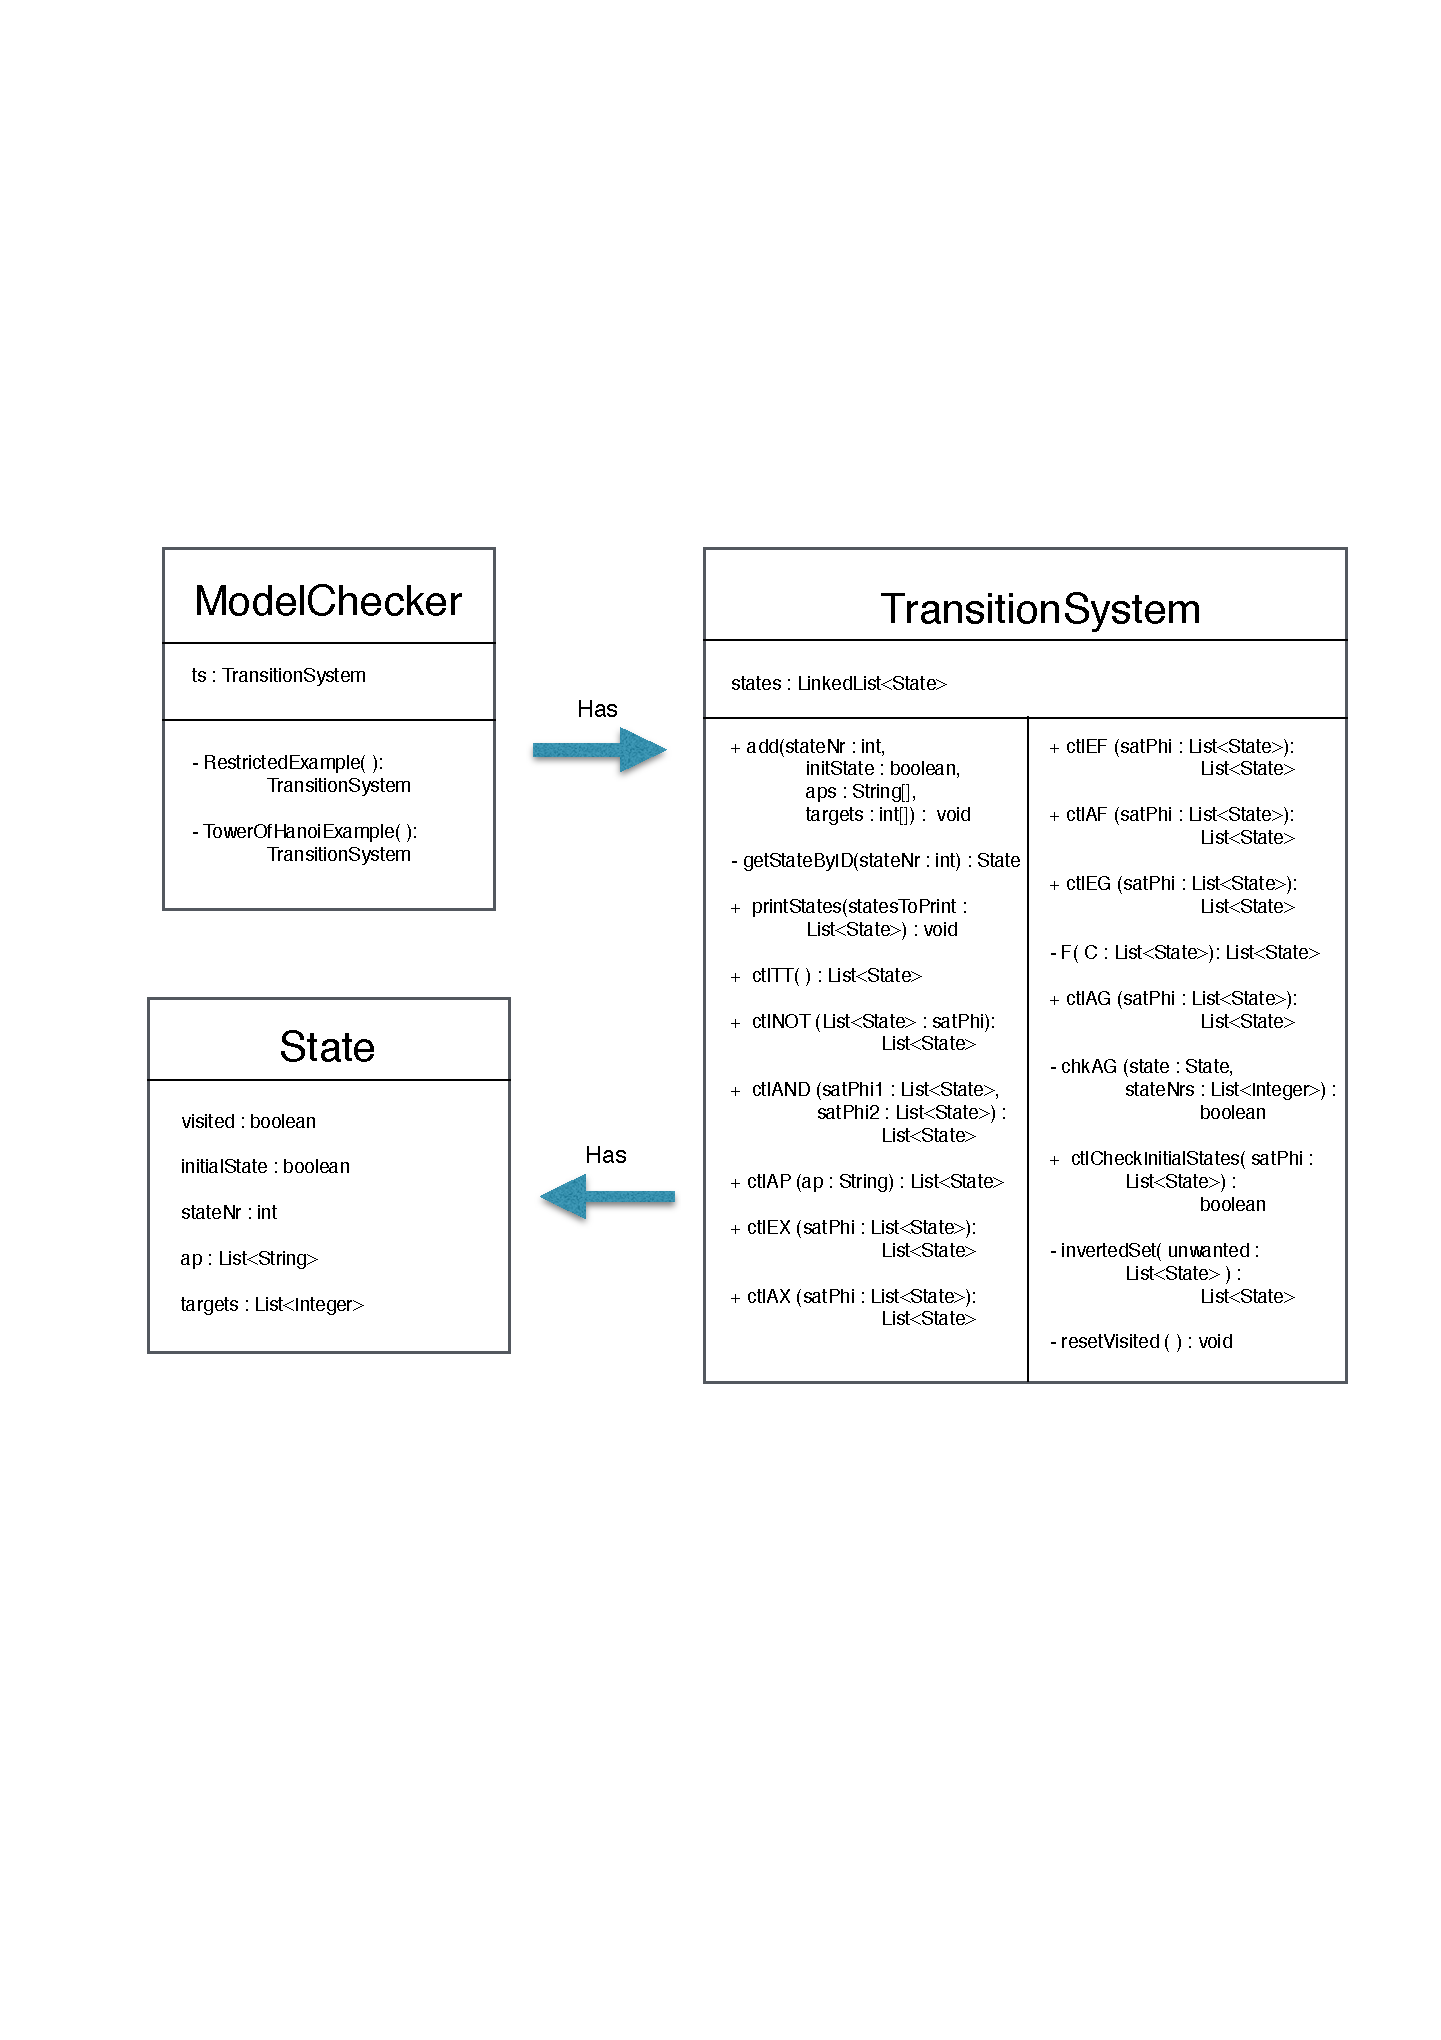
\includegraphics[width=\textwidth]{fig/classdiagram.pdf}
    \caption{Class diagram for the implementation.}
    \label{fig:classdiagram}
\end{figure}
